\documentclass{article}
\usepackage{graphicx}
\graphicspath{ {images/} }
\usepackage{listings}
\usepackage{color}

\definecolor{dkgreen}{rgb}{0,0.6,0}
\definecolor{gray}{rgb}{0.5,0.5,0.5}
\definecolor{mauve}{rgb}{0.58,0,0.82}

\lstset{frame=tb,
  language=Java,
  aboveskip=3mm,
  belowskip=3mm,
  showstringspaces=false,
  columns=flexible,
  basicstyle={\small\ttfamily},
  numbers=none,
  numberstyle=\tiny\color{gray},
  keywordstyle=\color{blue},
  commentstyle=\color{dkgreen},
  stringstyle=\color{mauve},
  breaklines=true,
  breakatwhitespace=true,
  tabsize=3
}
\begin{document}
	 1. The below screenshot shows both the result pushed to a webpage, as well as the output from running the command on the commandline.\\ 
	 	
	 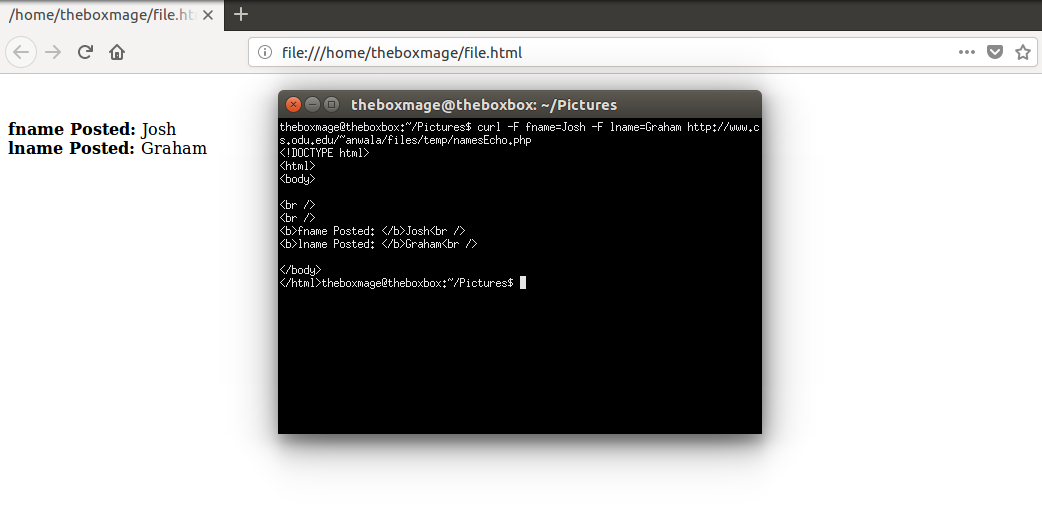
\includegraphics[scale=0.30]{Curl.png}	
 	 \pagebreak
	 \\2. Examples of how its run can be found in the txt files web1.txt web2.txt and web3.txt in the same directory as this file.

	 \begin{lstlisting}[language=Python]
import sys
import re
import requests
import urllib.request
from bs4 import BeautifulSoup


#Checking for at least one command line argument
if len(sys.argv) == 1:
	print('Not enough arguments')
	sys.exit()

#Downloading the information from the URL
resp = urllib.request.urlopen(sys.argv[1])
#Creating the BeautifulSoup Object to parse the webpage
soup = BeautifulSoup(resp, "html.parser")
print("Given URL: " )
print(sys.argv[1])
#Looping through all the links
for link in soup.find_all('a', attrs={'href': re.compile("^http:")}):
	#This cleanly and elegantly deals with any redirects.
	r = requests.head(link['href'], allow_redirects=True)
	# If the content type is application/pdf, its a pdf.
	if r.headers["Content-Type"] == "application/pdf":
		print("URL: ")
		print(r.url)
		print("Length in bytes: ")
		print(r.headers["Content-Length"])
		print()
	\end{lstlisting}
	
	\pagebreak
	3. The disconnected section really doesn't need an explanation. Tubes and tendrils only had one entry each, and they follow the path from the left value to the right one. The out values were harder for me, but they both stand relativley free. My largest issue was trying to figure out the difference between In and Scc. I'm still not overly confident that they are correct, but this is the closest I could get given the analogy.
	\begin{description}
	\item[IN]: I, P, O, M, N, L
	\item[SCC]: A, B, C, G
	\item[OUT]: H, D
	\item[TENDRILS]: I, K
	\item[TUBES]: L, D
	\item[DISCONNECTED]: E, F
	\end{description}



\end{document}
